\documentclass[11pt,a4paper]{article}
\usepackage[margin=2.3cm]{geometry}
\usepackage{amsmath,amssymb,amsthm}
\usepackage{graphicx}
\usepackage{booktabs}
\usepackage[hidelinks]{hyperref}
\usepackage{caption}
\captionsetup{font=small,labelfont=bf}
\newtheorem{proposition}{Proposition}
\newtheorem{lemma}{Lemma}
\newtheorem{corollary}{Corollary}
\theoremstyle{definition}
\newtheorem{definition}{Definition}
\theoremstyle{remark}
\newtheorem*{remark}{Remark}
\newcommand{\rc}{r_c}
\newcommand{\Rd}{R_d}
\newcommand{\Rb}{R_b}
\newcommand{\dd}{\mathrm{d}}
\newcommand{\Msun}{\mathrm{M}_\odot}

\title{On the origin of the factor $u$ of the P18 profile:\\
what is established, what is excluded, what remains open}
\author{B.~R. Parodi\\[2pt]\small companion note to \emph{From a primordial fluctuation to an idealised
rotation curve} (pf2irc), Sects.~2 and 6.5}
\date{2 November 2026}

\begin{document}
\maketitle

\begin{abstract}
\noindent The P18 profile is the singular isothermal sphere (SIS) times $u^2$, with
$u=1+(x-1)e^{-x}$ and $x=R/\rc$. Its form is empirical. This note collects what a first
inquiry into its origin has achieved. \emph{Established (exact).} $u$ is the unique
regular solution of the critically damped equation $u''+2u'+u=1$, $u(0)=0$, $u'(0)=2$, the
member $b=1$ of the regular family $u_b=1+(bx-1)e^{-x}$. If $\mu(x)$ is the mass fraction of
an exponential disc of scale length $\Rd=\rc$ inside $x$, then $u=1-\mu''$: P18 deviates
from the SIS by minus the radial gradient of the disc's mass per unit radius. The double
root of the equation is the composition of the exponential surface density with the
annulus factor $2\pi R$. The value $b=1$ is the only one for which the first-order part of
the density deviation carries no mass; the mass excess $c=\tfrac14=\int(u-1)^2\dd x$ is
purely second order, and the displaced mass splits exactly as
$x-m=2\mu'-\int_0^x\mu''^2$. At the temperature of the SIS, the Jeans equation requires
an anisotropy $\beta=1-xu'/u-m/x$: isotropic at the centre, mildly radial ($\beta\simeq0.15$)
between $0.5$ and $3\,\rc$, isotropic far out. \emph{Physical setting.} In the collapse of
the paper the dark matter stays nearly spherical ($v_{\rm rot}/\sigma\lesssim4\lambda$), while the gas
settles into a disc at its centrifugal radius, $\Rd/\rc\simeq0.7$--1.4. If the dwarfs kept
all their baryons, this disc would dominate the centre; about 90\% must be expelled.
\emph{Excluded.} Two numerical experiments test whether the expelled gas, through the
changing potential, can carve P18 out of the dark matter. Bursts in the paper's
self-similar shells flatten the cusp but act on the scale of the accretion front. Bursts of
an exponential disc in an isotropic SIS change little within the baryon budget and, even far
beyond it, expand the halo without removing the cusp: the centre of an SIS is shielded,
because the enclosed disc mass relative to the dark mass vanishes as $r/2\Rd$. \emph{Open.}
A core that forms while the disc grows during settling, so that the cusp never forms; and
torques of a rotating, non-axisymmetric disc. Both are left to a future project.
\end{abstract}

\tableofcontents
\bigskip

% =====================================================================
\section{Purpose and results}\label{sec:intro}

In the paper the total matter of a late-type dwarf galaxy follows the P18 profile,
\begin{equation}
  \rho(R)=\frac{v^2u(x)^2}{4\pi GR^2},\qquad u(x)=1+(x-1)\,e^{-x},\qquad x=\frac{R}{\rc},
  \label{eq:p18}
\end{equation}
with central density $\rho(0)=v^2/(\pi G\rc^2)$, enclosed mass $(v^2\rc/G)\,m(x)$ with
$m'=u^2$, and the closed form
$m(x)=x(1-e^{-x})^2+\tfrac14[1-(1+2x+2x^2)e^{-2x}]$. For $u\equiv1$ the profile is the
singular isothermal sphere (SIS). The \emph{displaced mass} $F(x)=x-m(x)$ is the mass that
P18 lacks inside $x$ compared with the SIS; $F'=1-u^2$. The paper takes the shape of $u$
from observations. This note asks where it could come from, and records what has been
achieved. Throughout, $D\equiv\dd/\dd x$, $g\equiv u-1$, masses are in units of $v^2\rc/G$
and specific energies in units of $v^2$ unless stated otherwise.

\begin{table}[h]
\centering\small
\caption{Results of this note and their status.}
\label{tab:results}
\begin{tabular}{@{}p{0.06\textwidth}p{0.62\textwidth}p{0.24\textwidth}@{}}
\toprule
Sect. & Result & Status\\
\midrule
2 & $u$ is the regular, critically damped solution with $b=1$ & theorem\\
2 & the isothermal sphere approaches the SIS underdamped in $\ln x$ & theorem, numbers\\
3 & $u=1-\mu''$ for an exponential disc with $\Rd=\rc$; the double root is profile $\times$ annulus & theorem\\
4 & $b=1$ $\Leftrightarrow$ no mass at first order; $c=\int g^2=\tfrac14$; $F=2\mu'-\int\mu''^2$ & theorem\\
5 & first order: shells displaced by $2R\,e^{-R/\rc}$, energy $2v^2e^{-R/\rc}\propto\Sigma_d$ & interpretation\\
6 & Jeans: $\beta=1-xu'/u-m/x$ at $\sigma_r^2=v^2/2$ & theorem (target, not cause)\\
7 & in the collapse: spherical dark matter, gas disc with $\Rd\approx\rc$, 90\% of the baryons expelled & estimates from the paper\\
8.1 & bursts in the self-similar shells: cusp flattened, but on the scale of the front & numerical, negative\\
8.2 & disc bursts in an isotropic SIS: no core; the centre is shielded & numerical, negative\\
8.3 & shielding: enclosed disc mass / dark mass $\to M_d\,r/(2\Rd)$ & theorem\\
\bottomrule
\end{tabular}
\end{table}

% =====================================================================
\section{The differential equation of $u$}\label{sec:ode}

\begin{proposition}\label{prop:ode}
$u(x)=1+(x-1)e^{-x}$ is the unique solution on $[0,\infty)$ of
\begin{equation}
  u''+2u'+u=1,\qquad u(0)=0,\qquad u'(0)=2.
  \label{eq:ode}
\end{equation}
Equivalently $g=u-1$ satisfies $(D+1)^2g=0$, $g(0)=-1$, $g'(0)=2$.
\end{proposition}
\begin{proof}
For $g=(x-1)e^{-x}$: $g'=(2-x)e^{-x}$, $g''=(x-3)e^{-x}$, so
$g''+2g'+g=(x-3+4-2x+x-1)e^{-x}=0$, and $u=1+g$ satisfies the inhomogeneous equation;
$u(0)=0$, $u'(0)=2$. A linear initial-value problem with constant coefficients has exactly one
solution.
\end{proof}

The characteristic polynomial is $(s+1)^2$: a double root, i.e.\ a \emph{critically damped}
oscillator, with $x$ in the role of time and $\rc$ as damping length.

\begin{proposition}[the regular family]\label{prop:family}
Every solution of $u''+2u'+u=1$ is $u=1+(A+Bx)e^{-x}$. The density $\rho\propto u^2/x^2$ is
finite at the centre if and only if $A=-1$. The regular solutions are therefore
\begin{equation}
  u_b(x)=1+(bx-1)\,e^{-x},\qquad u_b'(0)=b+1 .
  \label{eq:family}
\end{equation}
If the equation is written with a damping length $\lambda$ for the dimensional radius, its
regular solutions are $u_b(R/\lambda)$, with $\rho(0)=v^2(b+1)^2/(4\pi G\lambda^2)$; the core
radius defined by $\rho(0)=v^2/(\pi G\rc^2)$ is $\rc=2\lambda/(b+1)$. P18 ($b=1$) is the only
member with $\lambda=\rc$.
\end{proposition}
\begin{proof}
The general solution is the particular solution 1 plus the homogeneous solutions
$(A+Bx)e^{-x}$. Since $u(0)=1+A$, a finite limit of $u^2/x^2$ requires $1+A=0$; then
$u\simeq(B+1)x$ and $\rho(0)=v^2(B+1)^2/(4\pi G\lambda^2)$. Equating with
$v^2/(\pi G\rc^2)$ gives $\rc=2\lambda/(b+1)$, which equals $\lambda$ only for $b=1$.
\end{proof}

\begin{proposition}[properties]\label{prop:props}
(i) For $b>0$ the density crosses that of the SIS at $x=1/b$ only. (ii) $u_b$ exceeds 1
somewhere iff $b>0$; it then has one maximum, $1+b\,e^{-(b+1)/b}$ at $x=(b+1)/b$. (iii)
$m(x)-x\to c(b)=\int_0^\infty(u_b^2-1)\,\dd x=b^2/4+3b/2-3/2$, positive iff
$b>\sqrt{15}-3=0.873$. (iv) $u_b=(b+1)x-(b+\tfrac12)x^2+O(x^3)$, so the density falls linearly
at the centre unless $b=-\tfrac12$. For P18: crossing at $x=1$; maximum $u(2)=1+e^{-2}=1.135$;
$c=\tfrac14$; $F(1)=0.520$, $F=0$ at $x=3.29$, $F(\infty)=-\tfrac14$; the mass added outside
$\rc$ is $\int_1^\infty(u^2-1)\,\dd x=0.770$.
\end{proposition}
\begin{proof}
(i) $u_b-1$ has the sign of $bx-1$. (ii) $u_b'=(b+1-bx)e^{-x}$ vanishes once, at
$(b+1)/b$. (iii) With $\int_0^\infty x^ne^{-x}\dd x=n!$ and
$\int_0^\infty x^ne^{-2x}\dd x=n!/2^{n+1}$: $\int2g=2(b-1)$,
$\int g^2=b^2/4-b/2+1/2$; the sum is $c(b)$. (iv) Expand $e^{-x}$. The numbers are evaluated
in \texttt{code/identities.py}.
\end{proof}

\begin{proposition}[the isothermal sphere]\label{prop:emden}
The non-singular isothermal sphere, $\psi''+2\psi'/\xi=e^{-\psi}$, $\rho=\rho_0e^{-\psi}$,
linearised about its singular solution $e^{-\psi_s}=2/\xi^2$ (the SIS), obeys
$\delta_{ss}+\delta_s+2\delta=0$ in $s=\ln\xi$, with roots $-\tfrac12\pm\tfrac{\sqrt7}{2}i$.
Its density approaches the SIS as $\xi^{-1/2}\cos(\tfrac{\sqrt7}{2}\ln\xi+\varphi)$:
underdamped in $\ln R$, without a length scale.
\end{proposition}
\begin{proof}
Insert $\psi=\psi_s+\delta$, use $e^{-\psi}\simeq(2/\xi^2)(1-\delta)$, and change variable to
$s$; the equation has constant coefficients in $s$.
\end{proof}
For the same central density ($\rc=\sqrt8\,r_0$, $r_0^2=\sigma^2/4\pi G\rho_0$,
$\sigma^2=v^2/2$) the first maximum of $\rho/\rho_{\rm SIS}$ is 1.661 at $x=1.44$, the first
minimum 0.832 at $x=13.3$. Plain thermalisation therefore gives a scale-free ringing; a
mechanism for P18 must carry its own length.

% =====================================================================
\section{The disc representation of $u$}\label{sec:disc}

\begin{definition}
An exponential disc has $\Sigma(R)=\Sigma_0e^{-R/\Rd}$ and mass $M_d=2\pi\Sigma_0\Rd^2$. With
$x=R/\Rd$, its normalised enclosed mass is $\mu(x)=M_d(<R)/M_d$, and $\hat\Sigma=e^{-x}$ is its
normalised surface density.
\end{definition}

\begin{lemma}\label{lem:mu}
$\mu(x)=1-(1+x)e^{-x}$, $\mu'=x\,e^{-x}$, $\mu''=(1-x)e^{-x}$, $\mu'''=(x-2)e^{-x}$. Here
$\mu'=(\Rd/M_d)\,2\pi R\,\Sigma(R)$ is the mass of the annulus at $R$ per unit $x$.
\end{lemma}
\begin{proof}
$M_d(<R)=2\pi\Sigma_0\int_0^RR'e^{-R'/\Rd}\dd R'=2\pi\Sigma_0\Rd^2[1-(1+x)e^{-x}]$.
Differentiating: $\mu'=-e^{-x}+(1+x)e^{-x}=xe^{-x}$; $\mu''=e^{-x}-xe^{-x}$;
$\mu'''=-e^{-x}-(1-x)e^{-x}$. Further $\mu'=(\Rd/M_d)\,\dd M_d/\dd R$ and
$\dd M_d/\dd R=2\pi R\Sigma$.
\end{proof}

\begin{proposition}\label{prop:disc}
If $\Rd=\rc$, then
\begin{equation}
  u=1-\mu'' ,
  \label{eq:umu}
\end{equation}
equivalently $u=\mu+2\mu'$, and for the whole regular family
$u_b-1=-\mu''+(b-1)\,\mu'$.
\end{proposition}
\begin{proof}
$1-\mu''=1-(1-x)e^{-x}=1+(x-1)e^{-x}=u$. Since $\mu$ itself solves
$\mu''+2\mu'+\mu=1$ (it is the member $b=-1$ of the family), $1-\mu''=\mu+2\mu'$. Finally
$-\mu''+(b-1)\mu'=(x-1+bx-x)e^{-x}=(bx-1)e^{-x}=u_b-1$.
\end{proof}

\begin{corollary}[geometric reading]
With $\Rd=\rc$: P18 lies below the SIS ($u<1$) where the annulus mass $\mu'$ still grows
($x<1$); it crosses the SIS where the annulus mass is largest ($x=1$, $\mu''=0$); its
overshoot ($u>1$) lies where the annulus mass falls, and is largest at the inflection of
the annulus mass ($x=2$, $\mu'''=0$).
\end{corollary}

\begin{proposition}[origin of the double root]\label{prop:double}
$(D+1)\hat\Sigma=0$ and $(D+1)\mu'=\hat\Sigma$. Hence $(D+1)^2\mu'=0$, and
$(D+1)^2(u-1)=-(D+1)^2\mu''=-D(D+1)^2\mu'=0$.
\end{proposition}
\begin{proof}
$(D+1)e^{-x}=0$; $(D+1)(xe^{-x})=e^{-x}-xe^{-x}+xe^{-x}=e^{-x}$. $D$ commutes with $(D+1)^2$.
\end{proof}
The two equal ``relaxations in series'' of the critically damped equation are thus concrete:
the exponential fall of the surface density, and the annulus factor $2\pi R$, which makes the
annulus mass relax towards the surface density with the same length. The factor $x$ in
$xe^{-x}$ is the geometry of the annulus.

\begin{remark}
The solution space of Eq.~\eqref{eq:ode} is the affine space $1+\mathrm{span}\{e^{-x},xe^{-x}\}$,
so any two of its members are related by some first-order operator. The content of
Proposition~\ref{prop:disc} is therefore not that a disc \emph{causes} $u$, but that P18 and
an exponential disc share the same damped mode with the same length, if and only if $\Rd=\rc$.
\end{remark}

\begin{figure}[t]
\centering
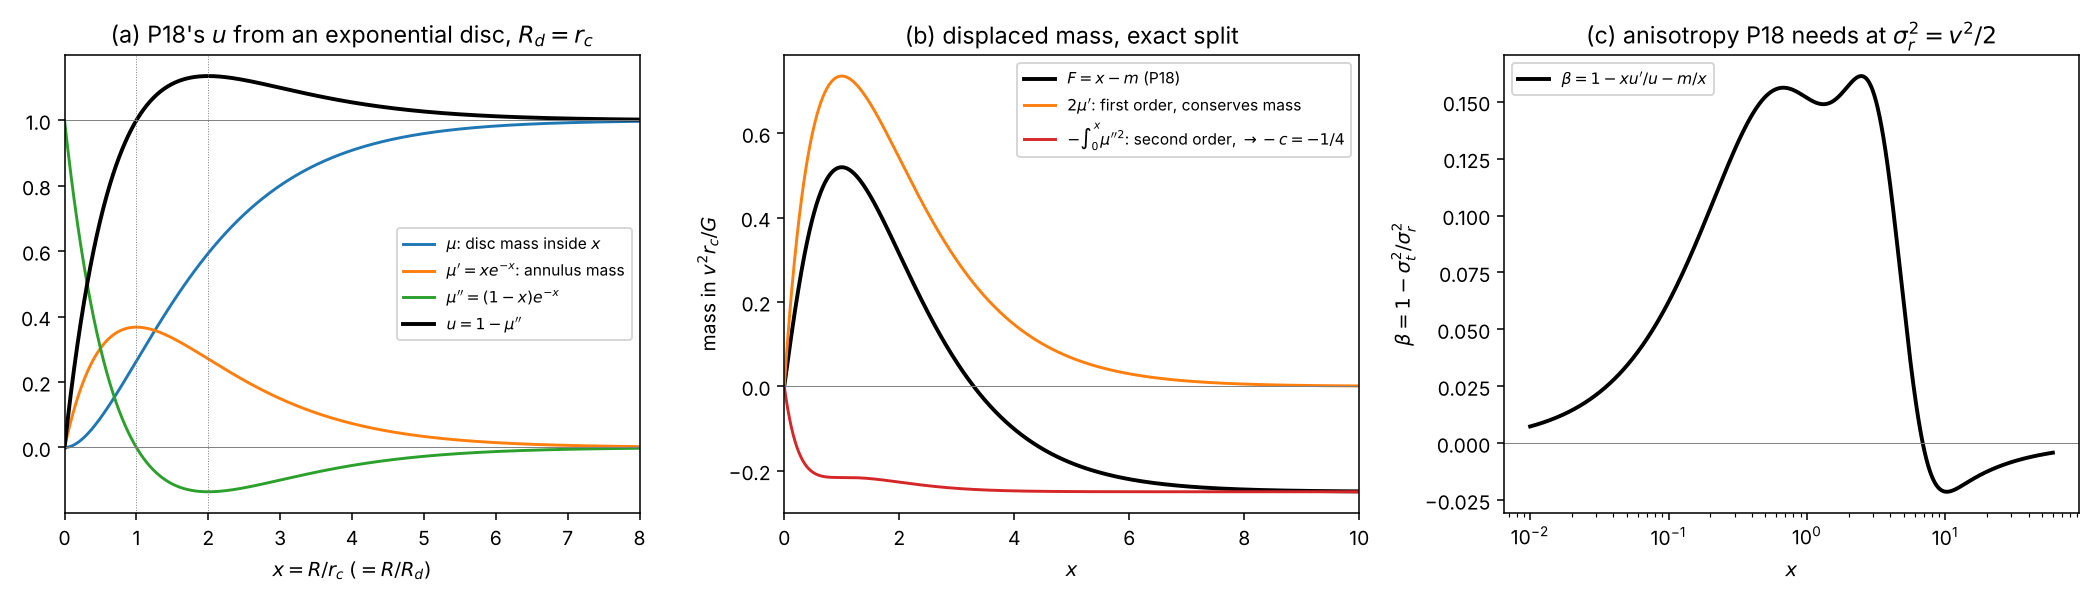
\includegraphics[width=\textwidth]{fig_disc.png}
\caption{(a) The exponential disc with $\Rd=\rc$: enclosed mass $\mu$, annulus mass $\mu'$, its
gradient $\mu''$, and $u=1-\mu''$. Dotted: the crossing ($x=1$) and the maximum ($x=2$). (b)
The exact split of the displaced mass, Proposition~\ref{prop:split}. (c) The anisotropy P18
requires at the temperature of the SIS, Proposition~\ref{prop:jeans}. Script:
\texttt{code/fig\_disc.py}.}
\label{fig:disc}
\end{figure}

% =====================================================================
\section{First-order mass conservation and the second-order excess}\label{sec:order}

Write $\rho/\rho_{\rm SIS}=u^2=1+2g+g^2$: a first-order and a second-order deviation.

\begin{proposition}\label{prop:order}
For the regular family, $\int_0^\infty g_b\,\dd x=b-1$ and
$\int_0^\infty g_b^2\,\dd x=b^2/4-b/2+1/2$, so that
$c(b)=2\int g_b+\int g_b^2$. Hence $b=1$ is the only member whose first-order deviation
carries no mass, and for P18 the mass excess is purely second order:
\begin{equation}
  c=\int_0^\infty(u-1)^2\,\dd x=\tfrac14 .
\end{equation}
\end{proposition}
\begin{proof}
$\int(bx-1)e^{-x}\dd x=b-1$; $\int(bx-1)^2e^{-2x}\dd x=b^2\tfrac14-2b\tfrac14+\tfrac12$.
\end{proof}

\begin{corollary}
Any profile of the form $u=1-\mu''$, with $\mu$ the enclosed-mass fraction of \emph{any} disc
whose annulus mass $\mu'$ vanishes at the centre and at infinity, conserves mass at first
order, since $\int_0^\infty\mu''\dd x=[\mu']_0^\infty=0$. The selection of $b=1$ is the
statement that the first-order deviation is the gradient of an annulus mass.
\end{corollary}

\begin{proposition}[exact split of the displaced mass]\label{prop:split}
\begin{equation}
  F(x)=x-m(x)=2\mu'(x)-\int_0^x\mu''(t)^2\,\dd t .
\end{equation}
The first term redistributes mass locally and vanishes far out; the second grows
monotonically to $c=\tfrac14$. At $\rc$: $0.736-0.216=0.520$.
\end{proposition}
\begin{proof}
$F'=1-u^2=-2g-g^2=2\mu''-\mu''^2$, and $F(0)=0=\mu'(0)$; integrate.
\end{proof}

% =====================================================================
\section{A first-order reading: displacement and energy}\label{sec:reading}

\emph{This section is an interpretation, valid where $|g|$ is small (beyond about
$1.5\,\rc$, where $|g|\le0.14$); it is not a derivation.} In an SIS,
$\dd M/\dd R=v^2/G$, so displacing every shell outward by $\xi(R)$ changes the enclosed mass by
$-(v^2/G)\,\xi$. The first-order part of $F$, $2\mu'$, therefore corresponds to
\begin{equation}
  \xi(R)=2\rc\,\mu'(x)=2R\,e^{-R/\rc}.
\end{equation}
A circular orbit in the SIS potential $v^2\ln R$ has specific energy $v^2(\tfrac12+\ln R)$, so
moving it by $\xi$ costs $v^2\xi/R$:
\begin{equation}
  \varepsilon(R)=\frac{v^2\,\xi}{R}=2v^2e^{-R/\rc}=2v^2\,\frac{\Sigma_d(R)}{\Sigma_d(0)} .
  \label{eq:eps}
\end{equation}
At first order, P18 is the SIS whose dark matter has received, at each radius, an energy per
unit mass proportional to the local surface density of an exponential disc with $\Rd=\rc$.
The amplitude is not free: a profile $u=1-A\mu''$ is regular ($u(0)=0$) only for $A=1$, which
gives $u'(0)=2$, $\rc=\Rd$, and $\varepsilon(0)=2v^2$. This agrees in order with the
requirement found in the companion note \emph{Halting and settling}, that the most bound
matter of the SIS be lifted by an energy of order $v^2$. The total,
$\int\varepsilon\,\dd M_{\rm SIS}=2v^2\cdot v^2\rc/G$, is $6\times10^{56}$\,erg for the median
dwarf ($v=73\,$km\,s$^{-1}$, $\rc=2.4$\,kpc): the supernova energy of about
$6\times10^7\Msun$ of stars at full coupling. Two cautions apply. At the centre the
displacement is non-linear ($\xi/R\to2$). And a collisionless response is not a local
displacement: each orbit averages over its radial range, so a local rule requires nearly
isotropic orbits.

% =====================================================================
\section{The anisotropy P18 requires}\label{sec:jeans}

\begin{proposition}\label{prop:jeans}
Let the radial velocity dispersion be constant at the SIS value, $\sigma_r^2=v^2/2$. Then P18
is an equilibrium of the spherical Jeans equation,
$\dd(\rho\sigma_r^2)/\dd R+2\beta\rho\sigma_r^2/R=-\rho\,GM/R^2$, if and only if
\begin{equation}
  \beta(x)=1-\frac{x\,u'}{u}-\frac{m}{x}.
  \label{eq:beta}
\end{equation}
$\beta\simeq\tfrac34x$ for $x\to0$ and $\beta\simeq-c/x$ for $x\to\infty$.
\end{proposition}
\begin{proof}
With $\sigma_r$ constant, $\sigma_r^2(\dd\ln\rho/\dd\ln R+2\beta)=-V^2$. From
Eq.~\eqref{eq:p18}, $\dd\ln\rho/\dd\ln R=2xu'/u-2$, and $V^2=v^2m/x$; inserting
$\sigma_r^2=v^2/2$ gives Eq.~\eqref{eq:beta}. Near the centre $u=2x-\tfrac32x^2+\dots$, so
$xu'/u=1-\tfrac34x+\dots$, and $m/x=O(x^2)$. Far out $u'\to0$ exponentially and
$m/x=1+c/x+\dots$.
\end{proof}

\begin{table}[h]
\centering\small
\caption{The anisotropy of Eq.~\eqref{eq:beta}. Maximum 0.161 at $x=2.47$; minimum $-0.021$
at $x=10.3$.}
\label{tab:beta}
\begin{tabular}{lcccccccccc}
\toprule
$x$ & 0.1 & 0.3 & 0.5 & 1 & 1.5 & 2 & 3 & 4 & 6 & 10\\
$\beta$ & 0.062 & 0.129 & 0.152 & 0.152 & 0.150 & 0.157 & 0.155 & 0.114 & 0.022 & $-0.021$\\
\bottomrule
\end{tabular}
\end{table}

At fixed temperature, P18 is the SIS plus a modest radial bias in the zone where it has been
rearranged, with isotropic orbits at the centre (as the distribution functions of
\emph{Halting and settling} also require). The Jeans equation can support many profiles with
a suitable $\beta$, so Eq.~\eqref{eq:beta} is a target for a mechanism, not an explanation.

\begin{remark}[general relativity]
The weak-field limit of the Einstein equations for a static sphere with radial and tangential
pressures, $p_r=\rho\sigma_r^2$ and $p_t=\rho\sigma_t^2$, is exactly this Jeans equation. At
$v=73\,$km\,s$^{-1}$, $v^2/c^2\simeq6\times10^{-8}$, so relativistic corrections to the core
are negligible. Spherical symmetry forces $p_\theta=p_\varphi$; a disc requires an axisymmetric
treatment, whose Newtonian form is the axisymmetric Jeans equations with $\sigma_R$,
$\sigma_\varphi$, $\sigma_z$ and a mean rotation.
\end{remark}

% =====================================================================
\section{The disc in the collapse of the paper}\label{sec:sth}

\emph{The dark matter stays spherical.} Each shell of the seed receives by turnaround the
specific angular momentum $j=2\sqrt2\lambda GM/v$ (mean over the mass inside it:
$\sqrt2\lambda GM/v$, paper Sect.~6.5). A collisionless shell contracts by a factor of only 2
between turnaround and halting, to $R\simeq GM/v^2$, so its rotation is at most
$j/R\simeq2\sqrt2\lambda v$, against $\sigma=v/\sqrt2$ in the SIS:
$v_{\rm rot}/\sigma\lesssim4\lambda=0.10$--0.20 for $\lambda=0.025$--0.05. The flattening,
of order $(v_{\rm rot}/\sigma)^2$, is a few per cent at most.

\emph{The gas forms a disc near $\rc$.} Gas radiates and contracts until it is supported by
rotation, at its centrifugal radius. With the paper's disc relation,
$\Rd/\rc=f_j\lambda y/\sqrt2$ (Mo--Mao--White), and the factor 1.06--1.4 found for the disc of
the seed (companion note \emph{The disc}), the core ratios $y$ of the paper's Table~1 give:
\begin{center}\small
\begin{tabular}{lccc}
\toprule
$\lambda$ & $y(z{=}0.5)$ & $\lambda y$ & $\Rd/\rc$ ($f_j=1$)\\
\midrule
0.025 & 39 & 0.98 & 0.69--0.97\\
0.035 & 34 & 1.19 & 0.84--1.18\\
0.05 & 28 & 1.40 & 0.99--1.39\\
\bottomrule
\end{tabular}
\end{center}
Since $y$ falls as $\lambda$ rises, $\lambda y$ varies only as $\lambda^{0.15\text{--}0.5}$, and
$\Rd/\rc$ stays of order unity. Both $\Rd$ and $\rc$ grow as $t$, so the ratio holds during
growth. The observed stellar discs have a median $\Rd/\rc=0.67$ with 0.30\,dex scatter.

\emph{The mass budget.} The cosmic baryon fraction is $\Omega_b/\Omega_m=0.157$. In units of
$v^2\rc/G$ (the SIS mass inside $\rc$ is 1):
\begin{center}\small
\begin{tabular}{lc}
\toprule
all baryons inside the front, $0.157\,y$ ($y=34$) & 5.35\\
baryons the dwarfs keep, 1.7\% of the mass inside the front (paper) & 0.58\\
mass P18 removes from inside $\rc$, $F(1)$ & 0.52\\
\bottomrule
\end{tabular}
\end{center}
A thin exponential disc has $V_{\max}^2=0.387\,GM_d/\Rd$ at $2.15\,\Rd$. With all baryons and
$\Rd=\rc$ the disc alone would reach $1.44\,v$, a baryon-dominated, peaked curve; with the
retained baryons, $0.47\,v$. About 90\% of the gas that passes through the disc must therefore
leave. Lifting it from $\rc$ to the front costs $v^2\ln y=3.5\,v^2$ per unit mass, in total
$16.8\,v^2(v^2\rc/G)$, eight times the $2\,v^2(v^2\rc/G)$ of Eq.~\eqref{eq:eps}. That the kept
disc is comparable to the displaced mass is noted, not claimed: the model's value depends on
$y$, which is uncertain by a factor of a few.

\emph{Two time scales.} The halted shells of the paper lie at the front,
$\Rb=\xi_bvt$ with $\xi_b=1/(1+3\pi/2)=0.175$; their gas continues inward to $\sim\rc=\Rb/y$.
The inflow therefore runs on the growth time $t$, while an orbit at $\rc$ takes
$2\pi\rc/v=2\pi\xi_b t/y=0.03\,t$: the dark matter in the core responds \emph{adiabatically}
to the growing disc and contracts. Star-formation bursts last tens of Myr, against an orbital
period at $\rc$ of about 200\,Myr for the median dwarf: the outflows act \emph{impulsively}.

\emph{The hypothesis tested.} (1) Dark matter and 16\% gas collapse; the dark matter halts near
the front, spherical. (2) The gas settles into a disc with $\Rd\approx\rc$, which supplies the
pattern $\Sigma_d\propto e^{-R/\rc}$ and, through Eq.~\eqref{eq:umu}, the critically damped
form. (3) Stars ignite in the disc, and about 90\% of the gas is expelled in cycles. (4) The
spherical dark matter answers this forcing with $\varepsilon\propto\Sigma_d$. (5) What remains
is P18 total matter. Steps (1)--(3) follow from the paper's numbers; step (4) is tested below.

% =====================================================================
\section{Numerical experiments}\label{sec:runs}

\subsection{Bursts in the self-similar shells}\label{sec:shells}

The earlier note \emph{u\_oscillator} (subfolder \texttt{u\_oscillator} of this package) adds to the paper's one-dimensional self-similar shells
(2000 shells, $\lambda=0.035$, $j=\sqrt2\lambda R_{\rm ta}$ at turnaround, units $G=v=1$) a
prescribed central baryonic Plummer sphere of mass $f_b\,\xi_f\,t$ ($\xi_f=0.2$), whose radius
jumps between $0.002\,t$ and $a_e\,t$ in cycles of length $P\,t$ (code:
\texttt{code/shells/fbshells.py}). The front lies at $\xi=R/vt\simeq0.21$, the model's core at
$\xi\simeq0.006$. Table~\ref{tab:shells} summarises the nine runs.

\begin{table}[h]
\centering\footnotesize
\setlength\tabcolsep{4pt}
\caption{Bursts in the self-similar shells (from the earlier note \emph{u\_oscillator}). Slope: dark-matter
density at $\xi=0.002$--0.006. $F$: displaced dark matter against the run without baryons.}
\label{tab:shells}
\begin{tabular}{lcccccc}
\toprule
run & $f_b$ & $a_e$ & $P$ & slope & peak of $F$ (at $\xi$) & $F<0$ beyond $\xi$\\
\midrule
reference & 0 & -- & -- & $-2.46$ & -- & --\\
fb05, fb10, fb20 & 0.05--0.20 & 0.05 & 0.05 & $-1.28$, $-0.77$, $-1.26$ & 0.04--0.09 (0.20--0.22) & --\\
fb05fast & 0.05 & 0.05 & 0.01 & $-1.02$ & 0.051 (0.20) & --\\
fb10far & 0.10 & 0.20 & 0.05 & $-1.44$ & 0.072 (0.22) & --\\
fb05ae02, ae01 & 0.05 & 0.02, 0.01 & 0.05 & $-1.17$, $-1.80$ & 0.035, 0.020 (0.20--0.22) & 0.61, 0.48\\
fb02ae01 & 0.02 & 0.01 & 0.05 & $-2.27$ & 0.006 (0.09)$^a$ & 0.28\\
\bottomrule
\end{tabular}

\smallskip
$^a$ Only 3--5 times the noise of $F$.
\end{table}

The bursts flatten the cusp and rearrange the dark matter with a P18-like shape (a single peak
of $F$ and, when the gas is confined, a single zone of accumulation), but always on the scale of
the front, about $35\,\rc$, never at $\rc$. On nearly radial orbits the displaced matter is
deposited near its apocentres, where the infall turns it round.

\subsection{Disc bursts in an isotropic SIS}\label{sec:discruns}

\emph{Model} (\texttt{code/discburst.py}). Dark matter: $2\times10^5$ particles in three
dimensions, initially an isotropic SIS with $v=1$ ($\rho=1/4\pi r^2$, Maxwellian velocities with
$\sigma=1/\sqrt2$), truncated at $R_{\rm out}=100$, with a spherical force from the enclosed
dark mass (Plummer softening $0.02$), leapfrog with $\Delta t=0.004$. Gas: an exponential disc
of scale length $\Rd=1$, entering through its spherically enclosed mass $M_d(t)\,\mu(r)$.
Schedule: relaxation for 10 time units; the disc is built up to the retained mass $M_{\rm lo}=0.5$
over $T_{\rm fill}=20$ (three orbital periods at $\Rd$); then bursts, each a linear filling by
$\Delta M$ over $T_{\rm fill}$ (adiabatic) followed by an instantaneous drop back to
$M_{\rm lo}$ (impulsive); finally $M_{\rm lo}$ is kept. All runs last 200 time units and are
compared, over 15 snapshots in the last 18 units, with the run without disc. Units
$G=v=\Rd=1$, so masses are in $v^2\Rd/G$.

\begin{table}[h]
\centering\small
\setlength\tabcolsep{4pt}
\caption{Disc bursts in an isotropic SIS (\texttt{code/analyse\_out.txt}). Expelled: total gas mass
removed by the bursts. Slope: dark-matter density at $R=0.05$--$0.2\,\Rd$ (reference $-2.04$).
$\rho/\rho_{\rm ref}$: dark matter against the run without disc. $r_c$: P18 fitted to dark matter
plus retained disc.}
\label{tab:discruns}
\begin{tabular}{lcccccc}
\toprule
run & bursts $\times\,\Delta M$ & expelled & slope & $\rho/\rho_{\rm ref}$ at $R=0.3,1,3\,\Rd$ & $\beta$ at $1,3\,\Rd$ & $r_c/\Rd$\\
\midrule
adiab (disc grown, kept) & -- & 0 & $-2.06$ & 1.12, 1.12, 1.06 & 0.01, 0.01 & 0.05\\
cyc03 & $7\times0.3$ & 2.1 & $-1.90$ & 1.12, 1.12, 1.06 & 0.01, 0.00 & 0.05\\
cyc06 & $7\times0.6$ & 4.2 & $-1.81$ & 1.09, 1.08, 1.05 & 0.00, 0.01 & 0.05\\
big3 & $3\times1.5$ & 4.5 & $-1.91$ & 1.09, 1.05, 1.00 & 0.05, 0.04 & 0.05\\
strong7 & $7\times3.0$ & 21 & $-1.97$ & 0.96, 0.66, 0.62 & 0.17, 0.25 & 0.04\\
\bottomrule
\end{tabular}
\end{table}

\begin{figure}[t]
\centering
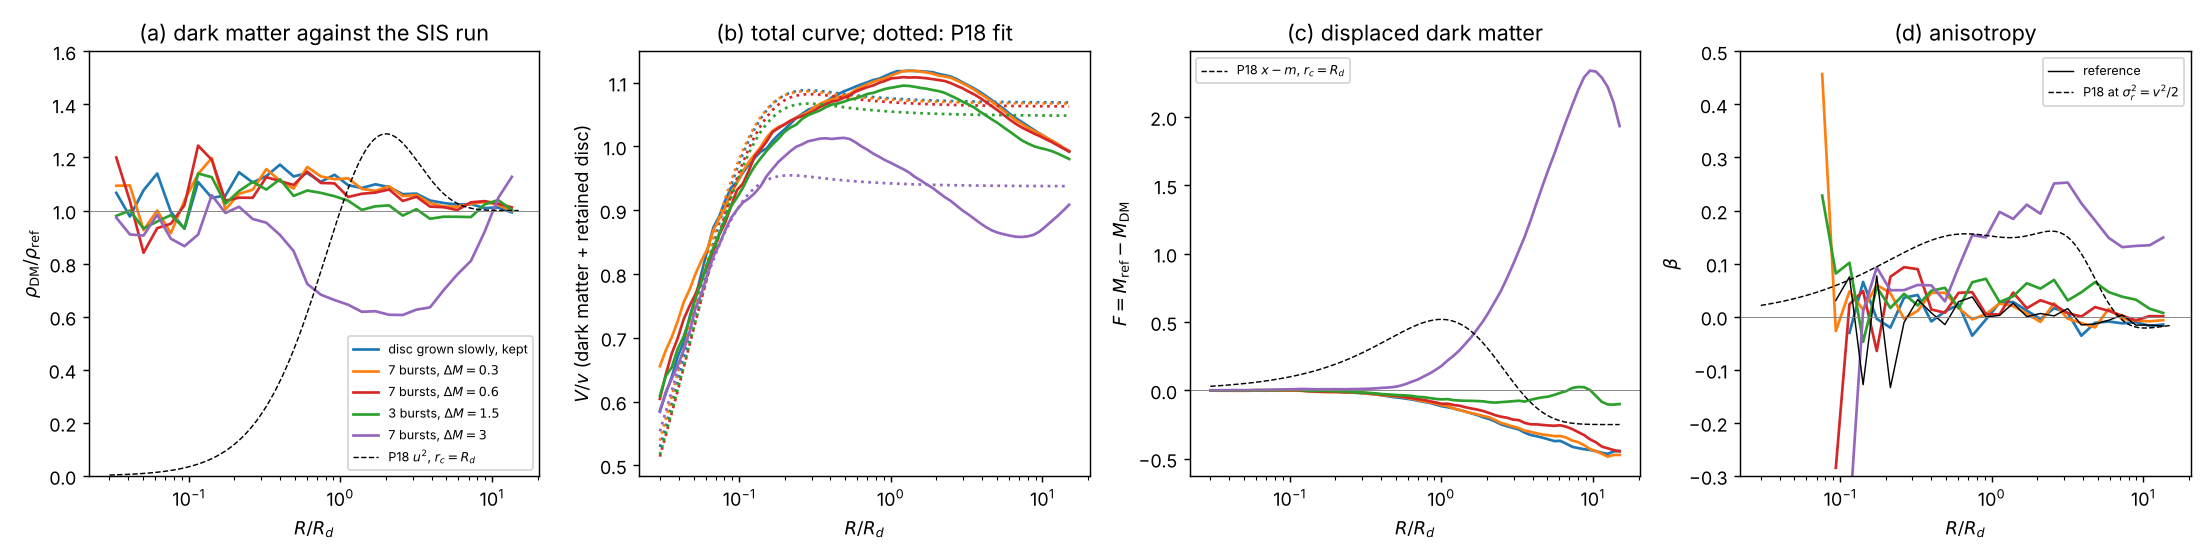
\includegraphics[width=\textwidth]{fig_runs.png}
\caption{Disc bursts in an isotropic SIS. (a) Dark-matter density against the run without disc,
with P18's $u^2$ for $\rc=\Rd$ (dashed). (b) Circular speed of dark matter plus retained disc;
dotted: P18 fits. (c) Displaced dark matter, with P18's $x-m$ (dashed). (d) Anisotropy, with the
reference run and Eq.~\eqref{eq:beta} (dashed). Script: \texttt{code/fig\_runs.py}.}
\label{fig:runs}
\end{figure}

\emph{Results} (Table~\ref{tab:discruns}, Fig.~\ref{fig:runs}).
\begin{enumerate}
\item \emph{Within the budget nothing much happens.} The retained disc, grown slowly, contracts
  the dark matter by about 10\% between $0.3$ and $2\,\Rd$. Bursts that expel up to 4.5 (the budget
  of Sect.~\ref{sec:sth} is 4.7) only partly undo this contraction; the inner slope changes from
  $-2.04$ to between $-1.8$ and $-1.9$. Fewer and larger bursts (big3) do somewhat better than
  many small ones with the same total, as expected for a heating of second order.
\item \emph{Strong forcing expands the halo but keeps the cusp.} With 21 units expelled (strong7),
  far beyond the budget, the dark matter is reduced by 35--40\% between 1 and $5\,\Rd$ and moved
  beyond $10\,\Rd$; the orbits there become radially biased ($\beta\simeq0.2$, the size
  Eq.~\eqref{eq:beta} asks for). But the inner slope stays at $-1.97$: no core, no crossing and no
  overshoot on the scale $\Rd$.
\item \emph{No P18 on the scale of the disc.} Fitted to dark matter plus retained disc, P18 returns
  $\rc\simeq0.05\,\Rd$ in every run, i.e.\ the softened cusp, not a core of size $\Rd$.
\end{enumerate}


\subsection{Why the centre is shielded}\label{sec:shield}

\begin{proposition}\label{prop:shield}
Let the dark matter be an SIS, $M_{\rm DM}(<r)=v^2r/G$, and let an exponential disc of mass
$\delta M$ and scale length $\Rd$ be added or removed, acting through its spherically
enclosed mass. Then the relative change of the enclosed mass, and of the gravitational force,
is
\begin{equation}
  \frac{\delta M\,\mu(r/\Rd)}{M_{\rm DM}(<r)}=\frac{G\,\delta M}{v^2\Rd}\,\frac{\mu(x)}{x}
  \simeq\frac{G\,\delta M}{v^2\Rd}\,\frac{x}{2}\qquad(x=r/\Rd\to0),
\end{equation}
and the change of potential across an orbit of size $r$ is, relative to $v^2$, of the same
order. If instead $M_{\rm DM}\propto r^2$ (an inner density $\propto r^{-1}$), the ratio tends
to a constant.
\end{proposition}
\begin{proof}
$\mu(x)=x^2/2+O(x^3)$ from Lemma~\ref{lem:mu}. The force ratio equals the enclosed-mass ratio
in spherical symmetry. The added force near the centre is the constant
$G\,\delta M/(2\Rd^2)$, so the potential changes across an orbit of size $r$ by
$G\,\delta M\,r/(2\Rd^2)$, which relative to $v^2$ is the same ratio. For
$M_{\rm DM}=kr^2$ the ratio tends to $G\,\delta M/(2k\Rd^2)$.
\end{proof}

The heating by a cycle of slow filling and sudden emptying is of second order in the potential
change, so it vanishes even faster towards the centre. A disc-shaped forcing therefore cannot
lift the most bound dark matter of an SIS by $\varepsilon(0)=2v^2$, as Eq.~\eqref{eq:eps}
requires, whatever its amplitude; the runs confirm this. Feedback cores in simulations start
from cusps with $\rho\propto r^{-1}$, for which the ratio stays finite. The collapse of the
paper, with the shells left to themselves, ends in an SIS-like cusp (paper, Appendix~H), which
is much harder to erase.

% =====================================================================
\section{Conclusions and open problems}\label{sec:conc}

\emph{Established.} The factor $u$ is the regular, critically damped solution with $b=1$; it
equals $1-\mu''$ for an exponential disc with $\Rd=\rc$; the double root is the composition of
the exponential surface density with the annulus factor; $b=1$ is singled out by mass
conservation at first order; the excess $c=\tfrac14$ is second order; and at the SIS temperature
P18 requires a radial bias $\beta\simeq0.15$ between $0.5$ and $3\,\rc$ with isotropic orbits at
the centre. In the paper's collapse a gas disc with $\Rd\approx\rc$ forms naturally, and most of
its gas must be expelled.

\emph{Excluded} (within the approximations stated). The dark matter cannot be given the P18
form by the changing potential of central gas bursts alone: in the self-similar shells the
rearrangement sits at the front; in an isotropic SIS a disc-shaped forcing cannot reach the
centre (Proposition~\ref{prop:shield}).

\emph{Open}, for a future project:
\begin{enumerate}
\item \emph{A core that never becomes a cusp.} If the disc grows while the halting shells pass
  through the centre, the SIS cusp need not form at all. This is assumption (A4) of the paper
  with a disc in it, and it fits the paper's picture of a core that grows with the galaxy. It
  requires the shell code with a disc grown during the collapse.
\item \emph{Torques instead of mass changes.} A rotating, non-axisymmetric disc (bar, spiral
  arms) exchanges angular momentum with dark-matter orbits through resonances; such torques are
  known to flatten cusps and isotropise orbits (Weinberg \& Katz 2002, ApJ 580, 627). A first test: test particles in an
  SIS plus a rotating bar of length $\sim\Rd$.
\item \emph{A local coupling rule.} Eq.~\eqref{eq:eps} asks for an energy per unit dark mass
  proportional to $\Sigma_d$. A naive feedback estimate gives energy per unit area $\propto\Sigma$
  but, divided by the dark column of an SIS ($\propto1/R$), an energy per unit mass
  $\propto R\Sigma$. Which physics, if any, gives $\Sigma$ itself is open.
\item \emph{The exact seed disc.} The disc of the seed is only nearly exponential (twice the
  exponential mass inside $0.5\,\Rd$, a sharp edge at $4.3\,\Rd$). Its $1-\mu''$ should be
  compared with $u$.
\end{enumerate}

\section*{References}
\noindent Background: Blumenthal et al.\ (1986, ApJ 301, 27) for adiabatic contraction;
Navarro, Eke \& Frenk (1996, MNRAS 283, L72) and Pontzen \& Governato (2012, MNRAS 421, 3464)
for cores from mass loss and potential fluctuations; Mo, Mao \& White (1998, MNRAS 295, 319) for
disc sizes; Binney \& Tremaine (2008, \emph{Galactic Dynamics}) for the Jeans equations.

\section*{Files in this package}
\begin{small}
\begin{tabular}{@{}lp{0.55\textwidth}@{}}
\texttt{code/identities.py} & checks of every formula and number of Sects.~2--7; output \texttt{identities\_out.txt}\\
\texttt{code/fig\_disc.py} & Fig.~\ref{fig:disc}\\
\texttt{code/discburst.py} & the disc-burst model of Sect.~\ref{sec:discruns}\\
\texttt{code/runall.py} & runs it (\texttt{python3 runall.py [names]}, two at a time); log \texttt{runs.log}\\
\texttt{code/analyse.py} & analysis (output \texttt{analyse\_out.txt})\\
\texttt{code/fig\_runs.py} & Fig.~\ref{fig:runs}\\
\texttt{code/shells/fbshells.py} & the self-similar shell code with central bursts of Sect.~\ref{sec:shells}; its nine runs, their analysis scripts, run files and figures are in the subfolder \texttt{u\_oscillator}\\
\end{tabular}
\end{small}

\medskip\noindent The subfolder \texttt{u\_oscillator} holds the earlier, more detailed note on
the differential equation and the burst experiment in the self-similar shells
(Sects.~2 and 8.1 here), with its code and run files. The run files of Sect.~\ref{sec:discruns} (about 13\,MB each) are not included; the runs take
about 10 minutes each and reproduce the numbers exactly with the seed set in the code.

\end{document}
